\section{Universality for Deterministic Matrices}
\label{sec:universality}

Recall the definition of puncturing (\Cref{def:puncturing}) and
of the \rrom~(\Cref{def:rom}).
Our main theorem in this section is:

\begin{theorem}
    \label{thm:universality-orthogonal}
    Let $\bH = \bH^{(n)}\in\R_{\sym}^{n\times n}$ be a sequence of symmetric orthogonal matrices such that
    \begin{align}
        \max_{1\le i\le j\le n} |\bmH[i,j]|\le n^{-\frac 12 + o(1)}\,.\label{eq:delocOrtho}
    \end{align}
    Then, the limiting traffic distribution of the puncturing of $\bm H$ 
    exists and equals that of the \rrom.
\end{theorem}

\noindent \Cref{thm:universality-orthogonal}
directly applies to $\bH$ being the sequence
of Walsh-Hadamard matrices, discrete sine
transform matrices, or discrete cosine 
transform matrices.
\Cref{thm:universality-orthogonal}
follows from the more general~\Cref{thm:universality-new} below, which applies
to symmetric matrices that are not
necessarily orthogonal, but have a
limiting diagonal distribution and 
satisfy
a generalized delocalization assumption.

\begin{assumption}
    \label{assumption:punctured}
    Let $\bH=\bH^{(n)} \in \R^{n \times n}_{\sym}$ and $\eps = \eps^{(n)}>0$.
    We introduce the assumptions:
    \begin{alignat}{2}
        \|\bH\|&\le 1, &&\label{eq:assNorm}\\[3.5mm]
        \max_{1\le i<j\le n} |\bW_\alpha(\bH)[i,j]|&\le \eps&\qquad&\text{for each open cactus $\alpha$ (\Cref{def:open-cactus})}, \label{eq:assOpen}\\
        \frac 1 {\sqrt n}\|\mathbf \Pi \bmw_\sigma(\bH) \|_2&\le \eps&\qquad&\text{for all $\sigma\in\calC_1$}, \label{eq:assOne}
    \end{alignat}
    where $\mathbf \Pi=\mathbf \Pi^{(n)} = \mathbf I - \frac 1n \bm 1 \bm 1^\top$ denotes the projection orthogonal to the all-ones direction. 
\end{assumption}

\noindent For example, one of the constraints of~\cref{eq:assOpen} is that $|\bH^k[i,j]| \leq \eps$ uniformly for all $k,n \in \N$ and distinct $i,j \in [n]$ (a bound which is uniform in $n,i,j$ but may depend on $k$ would also be sufficient, but we omit this for simplicity).



\begin{theorem}[Universality]
    \label{thm:universality-new}
    Let $\bH = \bH^{(n)}\in\R^{n\times n}_\sym$, $\bm A$ be the puncturing
    of $\bH$, and $\eps^{(n)} > 0$.
    \begin{enumerate}
        \item If $\bH$ satisfies~\cref{eq:assNorm,eq:assOpen}, then for all $\alpha\in \calE\setminus \calC$, 
        \[
            \frac 1n |z_\alpha(\bH)|\le O_\alpha\left( \varepsilon^{(n)} + \frac 1 {\sqrt n}\right)\qquad\text{and}\qquad\frac 1n |z_\alpha(\bA)|\le O_\alpha\left( \varepsilon^{(n)} + \frac 1 {\sqrt n}\right)\,.
        \]
        In particular, if $\eps^{(n)}=o(1)$, then
        both $\bH$ and $\bA$ satisfy the weak cactus property.
        \item If $\bH$ satisfies~\cref{eq:assNorm,eq:assOpen,eq:assOne}, then for all $\alpha\in \calA\setminus \calE$, 
        \[
            \frac 1n |w_\alpha(\bA)|\le \frac 1 {\sqrt n}\cdot \left(1 + \varepsilon^{(n)} \sqrt n\right)^{O_\alpha(1)}\,.
        \]
        In particular, if $\eps^{(n)} = n^{-\frac 12 + o(1)}$, then the right-hand side is $n^{-\frac 12 + o_\alpha(1)}$.
    \end{enumerate}
    Hence, if $\bH$ satisfies~\cref{eq:assNorm,eq:assOpen,eq:assOne} with $\eps^{(n)} = n^{-\frac 12 + o(1)}$, and the diagonal distribution of $\bH$ exists, then the traffic distribution of $\bA$ exists
    and is determined by the diagonal distribution of $\bH$.
\end{theorem}

\noindent We emphasized in the statement 
that all constants in the $O$
notations depend on $\alpha$.
We will drop this dependency in the rest
of the section.

\paragraph{Comparison with prior work.}
    In~\cite[Theorem 2.8]{wang2022universality}, the authors assume {\em (i)} delocalization of open cactuses
    (\cref{eq:assOpen}) and {\em (ii)} the existence of a limiting diagonal
    distribution. They show that, after conjugation by a randomly signed
    permutation matrix, the resulting ``semi-random'' matrix lies in the same
    universality class (in the sense of AMP dynamics) as an orthogonally
    invariant matrix with the same diagonal distribution.
    \Cref{thm:universality-new} shows that the same conclusion holds for
    deterministic matrices, if we replace random conjugation with puncturing.

    The universality result of \cite{wang2022universality} can also be extended in a black-box way to
    deterministic matrices, but only for GFOM with {\em odd} nonlinearities~\cite{dudeja2023universality,
    zhong2024approximate}. 
    This assumption lets one only consider the limiting traffic distribution evaluated on {\em Eulerian} diagrams. Under the same
    assumption, our proof would also 
    significantly simplify. Indeed, in~\Cref{thm:universality-orthogonal}, the number of monomials appearing in $w_\al(\bH)$ is $O(n^{|V(\al)|})$, and each term has magnitude $\max_{i,j\in [n]}|\bH[i,j]|^{|E(\al)|}\le n^{-|E(\al)|/2+o(1)}$, giving the upper bound $|w_\al(\bH)| \leq n^{o(1)}$ if $\al$ has minimum degree 4. It only remains to incorporate paths of degree-2 vertices, which simply compute $\bH^k\in \{\bm I, \bm H\}$ for some $k\ge 1$.
    
\subsection{Calculation of cactus diagrams and diagonal distribution}
\label{sec:diagonal-hadamard}

To apply~\Cref{thm:universality-new}, one needs to
compute the diagonal distribution of $\bH$ and small strengthenings of it
in order to verify~\Cref{assumption:punctured}.
Notice that the only diagrams involved in the assumptions are cactuses, so this is a much simpler task than calculating the entire traffic distribution.
In this subsection, we do this calculation directly to prove~\cref{thm:universality-orthogonal} assuming~\cref{thm:universality-new}.

Let $\bH$ be a delocalized orthogonal matrix
satisfying the assumption of~\cref{thm:universality-orthogonal}. Note that it
satisfies $\bH^2 = \bI$. Hence,~\cref{eq:assNorm} is automatic.
Next, we define the notion of {\em open cactus} appearing in~\cref{eq:assOpen}. An {open cactus} is
a matrix diagram with two roots such that merging the roots yields a cactus.
\begin{definition}
    \label{def:open-cactus}
    An { open cactus} is a graph obtained from
    a simple path by
    attaching vertex-disjoint cactuses to 
    each vertex of the path.
    Formally, $\alpha=(V(\alpha),E(\alpha))$
    is an open cactus if there exist $k\ge 2$,
    vertex-disjoint cactuses $\beta_1, \ldots, \beta_{k}$, and
    distinct vertices $u_1\in V(\beta_1), \ldots, u_{k}\in V(\beta_{k})$ with
    \[
        V(\alpha) = \bigcup_{i=1}^{k} V(\beta_i)\,,\quad E(\alpha) = \{\{u_i,u_{i+1}\}:i\in \{1,\ldots, k-1\}\}\cup \bigcup_{i=1}^{k} E(\beta_i)\,.
    \]
    We call $(u_1,u_{k})$ the {endpoints} of $\alpha$, and $(u_1, \ldots, u_k)$ the {base
    path} of $\alpha$.
    Unless specified otherwise, we will view
    an open cactus $\alpha\in\calA_2$ as a
    matrix diagram rooted at its two ordered endpoints.
\end{definition}

In general, if $\al$ is a matrix diagram and $\al^{\prime}$ is the scalar diagram formed by merging the roots of $\al$, then $\Tr(\bW_{\al}(\bA)) = w_{\al^{\prime}}(\bA)$.
For an open cactus $\al$, this $\al^{\prime}$ is a cactus, and so $w_{\al^{\prime}}(\bA)$ is one of the quantities whose limit is included in the diagonal distribution of $\bA$; further, all values of the diagonal distribution can be obtained in this way from the \emph{diagonal} entries of open cactus matrices.
From this perspective,
\cref{eq:assOpen} is a natural counterpart to the diagonal distribution since it concerns all of the \emph{off-diagonal} entries of the open cactus matrices.

We compute the open cactus matrices for $\bH$ in the following lemma.

\begin{lemma}\label{lem:diagonal-hadamard}
    Let $\sigma$ be an open cactus and let $\bH$ satisfy~\cref{eq:delocOrtho}.
    If all cycles in all of the hanging cactuses have even length, then $\bW_\sig(\bH) = \bI$ if the base path has even length and $\bW_\sig(\bH) = \bH$ if the base path has odd length. Otherwise, $\norm{\bW_\sig(\bH)} \leq n^{-\frac 12 + o(1)}$.
\end{lemma}

\begin{proof}
    First, the
    leaf 2-vertex-connected components of 
    $\sigma$
    consisting of cycles of even length
    can be iteratively removed without
    changing the value of $\bW_\sigma(\bH)$.
    This is because a hanging cycle of
    even length $k$ contributes $\text{diag}(\bH^{k}) = \text{diag}(\bI) = \bm 1$ in the 
    definition of $\bW_\sigma$.
    Therefore, if all cycles in all hanging cactuses have even length, then $\bmW_\sig(\bH) = \bH^\ell \in \{\bI, \bH\}$ where $\ell$ is the length of the base path.

    In the remaining case where $\sig$ has an odd cycle, we use induction.
    Let $\beta_1, \dots, \beta_k$ be the hanging cactuses of $\sig$.
    We convert each $\beta_i$
    into an open cactus diagram $\beta'_i$ by splitting the vertex at which $\beta_i$ meets $\sig$.
    With this notation, we have the matrix factorization:
    \begin{equation*}\label{eq:hadamard-cactus}
        \bW_{\sig}(\bH) = \diag(\bmW_{\beta'_1}(\bH)) \bH \diag(\bW_{\beta'_2}(\bH)) \bH  \ldots \bH\text{diag}(\bW_{\beta'_{k}}(\bH))\,.
    \end{equation*}

    The odd cycle in $\sig$ has either become an odd-length base path in some $\beta'_i$ or it continues
    to be an odd cycle in some $\beta'_i$.
    In the second case, by sub-multiplicativity of the spectral norm,
    \[
        \norm{\bW_\sig(\bH)} \leq \norm{\diag(\bW_{\beta'_i}(\bH))} \leq \norm{\bW_{\beta'_i}(\bH)} \le n^{-\frac 12 + o(1)}
    \]
    with the last inequality by induction.
    In the first case, we have $\bW_{\beta'_i}(\bH) = \bH$.
    Then 
    \[ \norm{\diag(\bW_{\beta'_i}(\bH))} = \norm{\diag(\bH)} \leq n^{-\frac 12 + o(1)}\] 
    by the delocalization assumption, and this case is also complete.
\end{proof}

We use the lemma to complete the proof of~\cref{thm:universality-orthogonal}.
\begin{proof}[Proof of~\Cref{thm:universality-orthogonal} from~\Cref{thm:universality-new}]
    \cref{eq:assNorm} holds automatically for $\bH$ a symmetric orthogonal matrix.
    Verifying~\cref{eq:assOpen},~\Cref{lem:diagonal-hadamard} implies that the off-diagonal entries of all open cactus matrices satisfy
    \[
        \max_{1\le i<j\le n} \left|\bW_\sig(\bH)[i,j]\right|\le \|\bW_\sig(\bH)\|\le n^{-\frac 12+o(1)}
    \]
    when $\sig$ has an odd cycle, and the remaining cases $\bW_\sig(\bH) = \bH$ or $\bW_\sig = \bI$ are easily checked.

    Next, each vector cactus diagram $\sig \in \cC_1$ satisfies $\bmw_\sig(\bH) = \diag(\bW_{\sig'}(\bH))$ where $\sig'$ is an open cactus obtained by splitting the root of $\sig$.
    By~\cref{lem:diagonal-hadamard} the diagonal of an open cactus matrix is either $\bm 1$ (in which case~\cref{eq:assOne} is satisfied with $\eps = 0$) or it satisfies
    \[
        \frac{1}{\sqrt{n}} \norm{\diag(\bW_{\sig'}(\bH))}_2 \le \norm{\diag(\bW_{\sig'}(\bH))}_\infty \leq n^{-\frac 12 + o(1)}\,,
    \]
    in which case~\cref{eq:assOne} is satisfied with $\eps = n^{-\frac 12 +o(1)}$.
    
    The diagonal distribution is computed by averaging the diagonal entries of open cactus matrices:
    \[
        \lim_{n\to\infty} \frac 1n w_\sigma(\bH) = \lim_{n\to\infty} \frac 1n \sum_{i=1}^n \bmW_{\sig'}[i,i] = \begin{cases}
            1 & \text{ if all cycles in $\sigma$ have even length}\\
            0 & \text{ otherwise}
        \end{cases}
    \]
    where on the left-hand side, we convert $\sigma\in\calC_0$ to an open cactus
    diagram $\sig'$ by rooting it arbitrarily and splitting the root.
    The right-hand side is by~\cref{lem:diagonal-hadamard}.
    That is, the diagonal distribution of $\bH$ is just the indicator function that all cycles of the cactus are even.

    Thus, we showed that~\cref{eq:assNorm,eq:assOpen,eq:assOne} hold and the diagonal distribution converges
    to the same fixed limit for any orthogonal matrix with delocalized entries. By~\Cref{thm:universality-new}, the
    traffic distribution of such matrices exists
    and is always the same.
    
    Finally, we show that the \rrom is also in this class, by showing that, after conditioning on a suitable high-probability event, the above argument applies to an \rrom matrix as well. 
    Let
    $\bH_{\rom} = \bQ \bD \bQ^\top$, where $\bQ$ is Haar-distributed and $\bD$ is diagonal
    with i.i.d. $\pm 1$ entries, independent of $\bQ$.
    \begin{claim}
        There exists $c>0$ such that for any $t>0$, 
        \begin{align}
            \max_{i,j\in [n]} |\bH_{\textnormal{\rom}}[i,j]|\le t^2 n^{-\frac 12}\label{eq:event-small-norm}
        \end{align}
        holds with probability at least $1-n^2 e^{-ct^2}$\,.
    \end{claim}
    \begin{proof}
    Since
    every entry of $\bQ$ is $O(n^{-1/2})$-subgaussian, by a union bound\[\max_{i,j\in [n]} |\bQ[i,j]|\le t n^{-\frac 12}\] holds with probability at least $1-n^2 e^{-\Omega(t^2)}$. Next, we have $\bH_{\textnormal{\rom}}[i,j] = \sum_{k=1}^n \bD[k,k] \bQ[i,k] \bQ[j,k]$, which, conditioned on $\bQ$, is a sum of independent
    random variables.
    By Hoeffding's bound, any fixed
    entry of $\bH_{\textnormal{\rom}}$ is $O(\sigma)$-subgaussian with parameter
    \[
        \sigma^2 \defeq \sum_{k=1}^n \bQ[i,k]^2 \bQ[j,k]^2\le \max_{i,j\in [n]} \bQ[i,j]^2\,,
    \]
    since every row of $\bQ$ has $\ell_2$-norm $1$. The conclusion follows from a union bound over all entries. 
    \end{proof}

    Fix $\alpha\in\calA$. Let $E_n$ denote the event~\cref{eq:event-small-norm},
    with $t = n^{o(1)}$. By the law of total expectation, we decompose
    \[
        \frac 1n \E w_\alpha(\bm \Pi \bH_{\textnormal{\rom}} \bm \Pi)
        =
        \frac 1n \E\!\left[w_\alpha(\bm \Pi \bH_{\textnormal{\rom}} \bm \Pi)\mid E_n\right]
        \Pr(E_n)
        +
        \frac 1n \E\!\left[w_\alpha(\bm \Pi \bH_{\textnormal{\rom}} \bm \Pi)\mid E_n^c\right]
        \Pr(E_n^c)\,.
    \]
    The left-hand side converges to the traffic distribution of the \rrom
    evaluated at $\alpha$. Moreover, since
    $\|\bm \Pi \bH_{\textnormal{\rom}} \bm \Pi\|\le 1$, we may crudely bound the
    second term by
    \[
        \frac 1n \E \left[w_\alpha(\bm \Pi \bH_{\textnormal{\rom}} \bm \Pi) \mid E_n^c\right]\cdot \Pr(E_n^c)\le n^{|V(\alpha)|-1} \Pr(E_n^c)\underset{n\to\infty}{\longrightarrow } 0\,.
    \]
    Since $\Pr(E_n)\underset{n\to\infty}{\longrightarrow} 1$, we deduce that
    \[
        \lim_{n\to\infty} \frac 1n \E \left[w_\alpha(\bm \Pi \bH_{\textnormal{\rom}} \bm \Pi) \mid E_n\right] = \lim_{n\to\infty} \frac 1n \E w_\alpha(\bm \Pi \bH_{\textnormal{\rom}} \bm \Pi)\,.
    \]
    Finally, on the event $E_n$, the matrix $\bH_{\textnormal{\rom}}$ satisfies the
    assumptions of~\Cref{thm:universality-orthogonal}. Consequently, the traffic
    distribution of punctured delocalized orthogonal matrices coincides with that
    of the \rrom, as desired.
\end{proof}

As a consequence of the above argument, the traffic distribution of the \rrom is specified implicitly as the solution to the following equations:
\begin{enumerate}
    \item For every $\alpha\in\calA\setminus \calE$, $\frac 1n \E w_\alpha(\bA) \underset{n\to\infty}{\longrightarrow}0$.
    \item For every $\alpha\in \calE\setminus \calC$, $\frac 1n \E z_\alpha(\bA) \underset{n\to\infty}{\longrightarrow}0$.
    \item For every $\sigma\in\calC$, $\frac 1n \E w_\sigma(\bA)\underset{n\to\infty}{\longrightarrow} 1$ if all cycles of $\sig$ are even and 0 otherwise.
\end{enumerate}
These equations determine a unique traffic distribution by~\cref{lem:eqDiffMobius}.
It is possible to give an explicit but much more complicated description using the Weingarten calculus, which we do in~\Cref{sec:puncturedWeingarten}.
However, the above characterization is arguably the conceptually clearer one, and we emphasize that it involves both the $w$- and $z$-bases.

We note also as a point of reference that the last part, the limiting values of cactuses in the $w$-basis, are the same as those for the (unpunctured) \rom, as follows from combining~\Cref{claim:rom-cumulants} with~\Cref{lem:diagonal-w-z}, and corresponds simply to the moments of the Rademacher distribution being 1 for moments of even order and 0 for ones of odd order.

\subsection{The fundamental theorem of graph polynomials}

The main proof of~\Cref{thm:universality-new} throughout the rest of the section relies on the
``fundamental theorem of graph polynomials'' of Bai and Silverstein~\cite{bai2010spectral}.
This result can be used to easily bound
2-edge-connected graph polynomials 
expressed in the $w$-basis, which is one reason that it is convenient to restrict to such diagrams in our definition of the weak cactus property.
The proof of the fundamental theorem uses a spectral bound on tensor powers of $\bA$; see \cite{mingo2012sharp} for another related result.

\begin{theorem}[{\cite[Theorems A.31 and A.32]{bai2010spectral}}]\label{thm:fundamental-theorem}
    For every $n\ge 1$, 
    $\alpha\in \calE\cup \calE_1\cup \calE_2$
    and collection of $n\times n$ symmetric matrices 
    $\bm \calA = (\bA_e)_{e\in E(\alpha)}$,
    \begin{alignat*}{2}
        \frac 1 n |w_\alpha(\bm \calA)|&\le \prod_{e\in E(\alpha)} \|\bA_e\| \quad&&\text{if $\alpha\in\calE$}, \\
        \|\bm w_\alpha(\bm \calA)\|_\infty&\le \prod_{e\in E(\alpha)} \|\bA_e\| \quad&&\text{if $\alpha\in\calE_1$}, \\
        \|\bW_\alpha(\bm \calA)\|&\le \prod_{e\in E(\alpha)} \|\bA_e\| \quad&&\text{if $\alpha\in\calE_2$}.
    \end{alignat*}
\end{theorem}

\noindent The result of~\cite{bai2010spectral} only covers scalar and matrix diagrams, but we provide a quick reduction
of the vector case to the scalar case.

\begin{proof}[Proof of vector case of~\cref{thm:fundamental-theorem}.]
    For all $q \ge 1$, we can diagrammatically express $\norm{\bw_\al(\bm \calA)}_{2q}^{2q}$ as the diagram formed by merging $2q$ copies of $\al$ at the root, and then forgetting the identity of the root to obtain a scalar diagram.
    Let $\al_{2q} = \alpha^{\oplus 2q}$ denote this diagram.
    The graph $\al_{2q}$ remains 2-edge-connected, therefore by the scalar case of the result we have:
    \[
        \norm{\bw_\al(\bm \calA)}_{2q}^{2q} = w_{\al_{2q}}(\bm \calA) \leq n \cdot \left(\prod_{e \in E(\al)} \norm{\bA_e}\right)^{2q}\,.
    \]
    Taking $q \to \infty$ with $n$ fixed, we obtain $\norm{\bw_\alpha (\bm \calA)}_\infty \leq \prod_{e \in E(\al)} \norm{\bA_e}$\,.
\end{proof}

We will apply the fundamental theorem by decomposing a general graph into its 2-edge-connected components,
which are joined together by a tree of bridge edges.
Decomposing diagrams into their 2-edge-connected components is also a fundamental idea in physics, where a 2-edge-connected Feynman diagram is called a ``1-particle-irreducible diagram''.


\subsection{Main structural lemma: Open cactus decomposition}

To prove the weak cactus property of~\Cref{thm:universality-new}, we begin by observing that
any 2-edge-connected non-cactus graph contains 
three edge-disjoint
paths between some pair of vertices.
How can we quantify that such a graph is a cactus plus excess edges?
We answer this question
by introducing the {\em open cactus decomposition}.
Our main structural result is that one can identify an ``extra'' open cactus subgraph inside any 2-edge-connected graph which is not a cactus, in the sense that the subgraph can be removed without spoiling 2-edge-connectedness.

\begin{proposition}
    \label{prop:open-cactus-decomposition}
    For any $\alpha\in\calE_1\setminus \calC_1$, there exist distinct $s,t\in V(\alpha)$ and
    an induced subgraph $\beta$ of $\al$ such that
    \begin{enumerate}
        \item $\beta$ is an open cactus with endpoints $\{s,t\}$.
        \item $\alpha\left[V(\alpha)\setminus (V(\beta)\setminus \{s,t\})\right]$ 
        is 2-edge-connected.
        \item $\rt(\al)\notin V(\beta)\setminus \{s,t\}$.
    \end{enumerate}
\end{proposition}

\begin{figure}[ht]
    \centering
    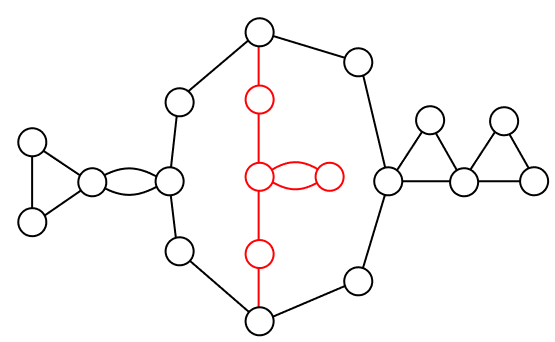
\includegraphics[width=0.35\linewidth]{images/2ec.png}
    \caption{Example for~\cref{prop:open-cactus-decomposition} of a 2-edge-connected graph which is not a cactus. If the open cactus in red is removed, the graph remains 2-edge-connected.}
    \label{fig:2ec}
\end{figure}

\noindent To prove~\Cref{prop:open-cactus-decomposition},
we will consider the last ear
in an {\em ear decomposition} of $\alpha$. We
prove a small variant of the classical
ear decomposition (see~\cite{robbins1939theorem} or~\cite[\S 5.3]{bondyMurty}) which lets us exclude a specified vertex from the internal vertices of the last ear.

\begin{lemma}
    \label{lem:ear-decomposition-lemma}
    Let $\alpha\in\calE_1$ be 2-edge-connected with at least 2
    vertices.
    There exists a path $\pi=(u_1, \ldots, u_k)$ in $\alpha$ with $k\ge 2$
    such that:
    \begin{enumerate}
        \item Each internal vertex $u_2, \ldots, u_{k-1}$ has degree 2 in $\alpha$.
        \item Each internal vertex $u_2, \ldots, u_{k-1}$ satisfies $u_i\neq \rt(\al)$.
        \item $u_1, \ldots, u_{k}$ are pairwise distinct, except possibly $u_1=u_k$.
        \item Removing internal vertices
        and edges of $\pi$ from $\alpha$
        leaves $\alpha$ 2-edge-connected.
    \end{enumerate}
\end{lemma}

\begin{proof}[Proof of~\Cref{lem:ear-decomposition-lemma}]
    Consider the following sequence $(\alpha_t)_{t\ge 0}$ of 2-edge connected subgraphs of $\alpha$:
    \begin{enumerate}
        \item Start from $\alpha_0$ being 
        any cycle of $\alpha$ containing $\rt(\al)$.
        \item Let $t\ge 0$. If $\alpha_t$ spans all vertices of $\alpha$, then stop.
        \item Otherwise, there exists
        $\{u_1,u_2\}\in E(\alpha)$ such that $u_1\in V(\alpha_t)$ and $u_2\notin V(\alpha_t)$. Since $\alpha$ is
        2-edge-connected, there exists a
        simple path
        $(u_2, \ldots, u_k)$ in $\alpha\setminus\{\{u_1,u_2\}\}$
        such that
        $u_i\notin V(\alpha_t)$ for all $2\le i\le k-1$, and $u_k\in V(\alpha_t)$.
        Set 
        \[
            \alpha_{t+1}=(V(\alpha_t)\cup \{u_2, \ldots, u_{k-1}\}, E(\alpha_t) \cup \{\{u_i,u_{i+1}\} : 1\le i<k\})\,.
        \]
    \end{enumerate}
    For any $t\ge 0$, $\alpha_t$ is 2-edge-connected.
    Therefore, if at the end of the algorithm $V(\alpha_t)=V(\alpha)$ but $E(\alpha_t)\neq E(\alpha)$, then any
    edge in $E(\alpha)\setminus E(\alpha_t)$
    is a length-1 path that satisfies the conclusion of the lemma.
    Otherwise, this means that $\alpha$ is
    obtained from
    $\alpha_{t-1}$ (which is 2-edge-connected) by adding a path of
    internal degree-2 vertices in $\alpha$
    which must all 
    be distinct from $\rt(\al)\in V(\alpha_0)\subseteq V(\alpha_{t-1})$. This concludes the proof.
\end{proof}


\begin{proof}[Proof of~{\Cref{prop:open-cactus-decomposition}}]
    Starting with the graph $\alpha$, consider the following procedure:
    \begin{enumerate}
        \item Delete all self-loops in $\alpha$.
        \item If no leaf 2-vertex-connected
        component (i.e., a 2-vertex-connected
        component meeting the rest of the graph
        at a single articulation point)
        consists of a single cycle,
        then stop.
        \item Otherwise, choose an arbitrary
        such component. Let $v$ be the articulation point connecting this component to the rest of graph. Delete all edges 
        of this component
        from the graph.
        \item Delete newly isolated vertices; exactly
        one vertex of the component remains, namely $v$. Since
        $\alpha\notin \calC_1$, the procedure
        does not delete the entire graph.
    
        \item If the root was removed in Step 4, set $v$ as the new root of the diagram.
        \item Return to Step 1.
    \end{enumerate}
    Call $\beta\in\calA_1$ the
    resulting rooted graph. Note that $\beta$
    is still 2-edge-connected, so
    by~\Cref{lem:ear-decomposition-lemma}, we can find a path
    $\pi = (u_1, \ldots, u_k)$ in $\beta$
    with internal degree-2 vertices. $\pi$ 
    cannot be a cycle because of our
    initial step of removing cyclic 2-vertex-connected components.
    Therefore, $\pi$ is a simple
    path and the root of $\beta$ is not an
    internal vertex of $\pi$.

    \begin{observation}\label{obs2-open}
        For $2\le i<k$, let $\sigma_i$ be the connected
        component of $u_i$ in $\alpha\setminus E(\pi)$. Then $\alpha' \defeq \pi\cup \sigma_2\cup \ldots \cup \sigma_{k-1}$ is
        an open cactus in $\alpha$ with endpoints $u_1,u_k$. Moreover, $\rt(\alpha)$
        is not an internal vertex of the open cactus.
    \end{observation}

    \begin{proof}
        $\pi$ is a simple
        path in $\beta$, and adding back loops and
        cyclic 2-vertex-connected components we removed from $\alpha$, we obtain an open cactus.
        The recursive pruning procedure we used 
        to transfer
        the root ensures that $\rt(\alpha)$
        is not in any of the cyclic 2-vertex-connected
        components that are added to $\pi$.
    \end{proof}

    \begin{observation}\label{obs1-open}
        $\alpha\left[V(\alpha)\setminus (V(\alpha')\setminus \{u_1,u_k\})\right]$
        is 2-edge-connected.
    \end{observation}

    \begin{proof}
        By~\Cref{lem:ear-decomposition-lemma},
        $\beta\left[V(\beta)\setminus \{u_2, \ldots, u_{k-1}\}\right]$ is 2-edge-connected.
        Adding 2-vertex-connected cyclic components
        to this graph preserves 2-edge-connectivity.
    \end{proof}
    \noindent
    \Cref{obs2-open} and~\Cref{obs1-open} conclude
    the proof of~\Cref{prop:open-cactus-decomposition}.
\end{proof}

\subsection{The effect of puncturing}

The main result of this subsection is:

\begin{proposition}
    \label{prop:to-punctured}
    Let
    $\bH \in \R^{n \times n}_\sym$ such that $\|\bH\|\le 1$ and $\bm u\in\R^n$ be a unit vector. Denote by $\bA = (\bI - \bm u \bm u^\top) \bH (\bI - \bm u\bm u^\top)$.
    Then for any open cactus $\alpha\in\calA_2$,
    \[
        \|\bW_\alpha(\bA) - \bW_\alpha(\bH)\|_{\textnormal F}\le |E(\alpha)|\cdot \|\bm A - \bm H\|_\frob\le 3|E(\alpha)|\,.
    \]
\end{proposition}

We deduce in the following that puncturing does not change the diagonal distribution.
In particular, matrices such as the \rom and the \rrom have the same diagonal distribution.

\begin{corollary}
    \label{cor:cactus-puncturing-same}
    Let $\bH$ and $\bA$ be as in~\Cref{prop:to-punctured}. Then for any $\sigma\in\calC_1$
    \[
        \|\bw_\sigma(\bH) - \bw_\sigma(\bA)\|_2 \le O(1)\,,
    \]
    and for any $\sigma\in \calC$,
    \[
        \frac 1n |w_\sigma(\bH) - w_\sigma(\bA)| \le O\left(\frac 1 {\sqrt n}\right)\,.
    \]
\end{corollary}

\begin{proof}[Proof of~\Cref{cor:cactus-puncturing-same} from~\Cref{prop:to-punctured}]
    Except for the case where $\sigma \in \cC_1$ has one vertex (in which case the statement holds because the diagonal entries are bounded), $\rt(\sigma)$ has degree $\ge 2$. Create
    two copies $r_1,r_2$ of $\rt(\sigma)$ and re-assign the edges
    incident to $\rt(\sig)$ to $r_1$ or $r_2$ in such a way that $r_1$ and $r_2$
    have degree at least $1$. The resulting
    graph is an open cactus $\alpha$ with endpoints $r_1$ and $r_2$ such that merging
    these endpoints yields back $\sigma$.
    Hence,
    \[
        \|\bw_\sigma(\bH) - \bw_\sigma(\bA)\|_2 = \|\textnormal{diag}(\bW_\alpha(\bH)) - \textnormal{diag}(\bW_\alpha(\bA))\|_{\textnormal F}\le O(1)\,.
    \]
    The second statement then follows from Cauchy-Schwarz:
    \[
        |w_\sigma(\bH)-w_\sigma(\bA)| = |\langle \bm 1, \bw_\sigma(\bH)-\bw_\sigma(\bA)\rangle| \le \sqrt n \cdot  \|\bw_\sigma(\bH) - \bw_\sigma(\bA)\|_2\le O(\sqrt n)\,.
    \]
    This concludes the proof.
\end{proof}

However, $\bH$ and its punctured version $\bA$ may  
{\em not} have the same traffic distribution, even on scalar open
cactuses.
Thus, the diagonal distribution (i.e., the values of cactus diagrams) is not sensitive to the behavior of $\bH$ in any single direction $\bu$, while some diagrams in the traffic distribution \emph{are} sensitive to the behavior in the $\bm 1$ direction.

\begin{example}[Puncturing of the Walsh-Hadamard matrix]\label{ex:puncture-hadamard}
    Let $\bH^{(n)}$ be the normalized
    Walsh-Hadamard matrices (\Cref{def:hadamard}). Then for the 2-path diagram $\alpha$ (which is an open cactus),
    \[
        \frac 1n (w_\alpha(\bH) - w_\alpha(\bA)) = \frac 1n \langle \bm 1, (\bH^2 - \bA^2) \bm 1\rangle  \underset{n\to\infty}{\longrightarrow} 1\,.
    \]
    This does not contradict~\Cref{prop:to-punctured}: $\bE = \bW_\alpha(\bH) - \bW_\alpha(\bA)$ indeed satisfies
    \[
        \sum_{i,j=1}^n \bE[i,j]^2 \le O(1)\quad \text{ and }\quad \left|\sum_{i,j=1}^n \bE[i,j] \right| = \Omega(n)\,.
    \]

\end{example}

In general, as the following example demonstrates, the off-diagonal structure of the error matrix
$\bE = \bW_\alpha(\bH) - \bW_\alpha(\bA)$ in~\Cref{prop:to-punctured} may
be intricate. 
In the following example, $\bE$ has
entries of magnitude $\Omega(1)$, even though its
Frobenius norm remains bounded.

\begin{example}[Puncturing of the DST matrix]
        Let $\bH^{(n)}$ be the discrete sine transform matrices (\Cref{def:dst}).
        Then for any fixed odd $i\ge 1$, the 
        normalized sum of the $i$th row of
        $\bH^{(n)}$ is
        \[
            \frac {1} {\sqrt n} \sum_{j=1}^n \bH[i,j] = (\sqrt 2+o(1)) \int_0^1 \sin(\pi i t) \,\d t \underset{n\to\infty}{\longrightarrow} \frac {2 \sqrt 2} {i\pi }\,.
        \]
        Consider the 2-path diagram $\alpha$. While the
        off-diagonal entries of $\bW_\alpha(\bH) = \bH^2$
        vanish (since $\bH$ is a symmetric
        orthogonal matrix), on the other hand, for any
        fixed distinct odd numbers $i,j\ge 1$, 
        \[
            \bW_\alpha(\bA)[i,j] = (\bA^2)[i,j]\underset{n\to\infty}{\longrightarrow} -\frac {8} {ij \pi^2}\,,
        \]
        which is $\Omega(1)$ for constant $i\neq j$.
\end{example}

\noindent The proof of~\Cref{prop:to-punctured}
relies on expanding $\bA$ in terms of
$\bm u\bm u^\top$ and $\bH$. All rank-1 terms
can be neglected thanks to the following
lemma:

\begin{lemma}
    \label{lem:low-rank}
    Let $\alpha$ be an open cactus, $e^*\in E(\alpha)$, and $\bm \calA = (\bA_e)_{e\in E(\alpha)}$
    be a collection of matrices such
    that $\|\bA_e\|\le 1$ for all
    $e\in E(\alpha)\setminus \{e^*\}$. Then,
    \[
        \|\bW_\alpha(\bm \calA)\|_{\textnormal F}\le \|\bA_{e^*}\|_{\textnormal F}\,.
    \]
\end{lemma}


\begin{proof}
    We first
    run a pruning procedure that iteratively removes parts of $\alpha$ not containing
    $e^*$, without decreasing the
    Frobenius norm of $\bW_\alpha(\bm \calA)$
    during the procedure.
    To this end, we use repeatedly the standard inequalities:

    \begin{claim}    
    \label{claim:frobenius-product}
        $\|\bmM_1 \bmM_2\|_\frob\le \|\bmM_1\|_\frob \|\bmM_2\|$.
    \end{claim}
    
    \begin{claim}
    \label{claim:frobenius-hadamard}
    $\|\bmM_1 \odot \bmM_2\|_\frob\le \|\bmM_1\|_\frob\cdot  \max_{1\le i,j\le n} \left|\bmM_2[i,j]\right|\le \|\bmM_1\|_\frob \|\bmM_2\|$, where $\odot$ denotes entrywise or Hadamard product.
    \end{claim}
    
    Initially, let $u_{\textnormal L}$
    be one of the endpoints of $\alpha$.
    \begin{enumerate}
        \item If $e^*$ belongs to a
        cactus hanging from $u_{\textnormal L}$, then stop.
        \item Otherwise, remove
        the cactus hanging from $u_{\textnormal L}$ from the diagram. Using~\Cref{claim:frobenius-hadamard} and~\Cref{thm:fundamental-theorem} 
        (the spectral norm of the cactus matrix
        diagram with a double root at $u_{\textnormal L}$ is at most 1), this does not 
        decrease
        the Frobenius norm. 
        \item At this point, $u_{\textnormal L}$ must have degree equal to 1 in the current graph. If $e$ is the edge 
        adjacent to $u_{\textnormal L}$, then stop. 
        \item Otherwise, remove the edge
        adjacent to $u_{\textnormal L}$.
        By~\Cref{claim:frobenius-product} and the assumption, this does not decrease the
        Frobenius norm. Set $u_{\textnormal L}$ to be the
        vertex that was adjacent to
        $u_{\textnormal L}$, and go
        back to the first step.
    \end{enumerate}
    Then, apply the symmetric procedure
    from the other endpoint $u_{\textnormal R}$ of $\alpha$. At
    this point, there are two cases. If $u_{\textnormal L} \neq u_{\textnormal R}$, then the resulting graph
    must consist of the single edge
    $e^* = \{u_{\textnormal L}, u_{\textnormal R}\}$, so we get
    the desired upper bound on the Frobenius norm. Therefore, we
    assume from now on that $u_{\textnormal L} = u_{\textnormal R}$.
    
    The resulting graph must be a cactus rooted at $u_{\textnormal L} = u_{\textnormal R}$, and $e^*$ is
    one of the edges of this cactus.
    If there are several cycles
    incident to $u_{\textnormal L}$,
    we use again~\Cref{claim:frobenius-hadamard} and~\Cref{thm:fundamental-theorem} to remove all such cycles
    not containing $e^*$ without
    decreasing the Frobenius norm.
    
    Finally, we bound the Frobenius norm of
    the diagonal cactus matrix rooted at
    $u_{\textnormal L}$ by the
    Frobenius norm of an open cactus
    obtained by creating two copies
    of the root and turning the unique
    cycle hanging at $u_{\textnormal L}$ into a simple path between
    these two copies (we used a similar procedure
    in~\Cref{cor:cactus-puncturing-same}). We claim that this open cactus has strictly less edges
    than the one we started with
    before running the pruning procedure. Indeed,
    the base path had at least one edge, which
    was removed during the pruning stage when
    $u_{\textnormal L} = u_{\textnormal R}$ at the end. We
    conclude by induction on the
    number of edges of the open cactus.
\end{proof}

\begin{proof}[Proof of {\Cref{prop:to-punctured}}]
    We replace iteratively $\bm H$ by
    $\bm A$ in the graph polynomial $\bm W_\alpha(\bm H)$: let $e_1, \ldots, e_{|E(\alpha)|}$
    be the edges of $\alpha$, and write
    \[
        \bm W_\alpha(\bm A) - \bm W_\alpha(\bm H) = \sum_{i=1}^{|E(\alpha)|} \bm W_\alpha(\bm \calA_{i})\,,
    \]
    where $\bm \calA_i[e_j] = \bm H$ if $j<i$, $\bm \calA_i[e_j] = \bm A$ if $j>i$, and $\bm \calA_i[e_i] = \bm A - \bm H$.
    For each $i\in [|E(\alpha)|]$, we apply~\Cref{lem:low-rank} with $e^* = e_i$.
    We have $\|\bm A\|\le 1$ and $\|\bm H\|\le 1$
    so the assumptions of the lemma are satisfied, and we deduce
    \[
        \|\bm W_\alpha(\bm \calA_i)\|_\frob\le \|\bm A - \bm H \|_\frob\,,
    \]
    and by the triangle inequality
    \[
        \|\bm W_\alpha(\bm A) - \bm W_\alpha(\bm H)\|_\frob\le |E(\alpha)|\cdot \|\bm A - \bm H\|_\frob\,.
    \]
    Finally, we have
    \[
        \bA - \bH = \langle \bu,\bH \bu\rangle \bu\bu^\top - (\bH \bu\bu^\top + \bu\bu^\top \bH)\,.
    \]
    Since $\|\bH\|\le 1$ and $\bu$ is a unit vector, we have $|\langle \bu, \bH \bu\rangle|\le 1$ and $\|\bH \bu\|_2\le 1$, so $\|\bm A - \bm H\|_{\textnormal F}\le 3$.
\end{proof}

\subsection{Support of the \texorpdfstring{$z$}{z}-basis}

Let $\bH=\bmH^{(n)}$ be a family of matrices
satisfying~\cref{eq:assNorm,eq:assOpen}
and $\bmA=\bmA^{(n)}$ be their puncturing.
The main result of this subsection is
that $\bA$ and $\bH$ satisfy the weak cactus
property, that is, their traffic 
distribution in the $z$-basis is supported on
cactuses and graphs with bridges.

\begin{proposition}
    \label{prop:Z-support}
    For any $\alpha\in \calE\setminus \calC$,
    \[
        \frac 1n |z_\alpha(\bH)|\le O\left(\eps + \frac 1 {\sqrt n}\right)\quad\text{and}\quad \frac 1n |z_\alpha(\bA)|\le O\left(\eps + \frac 1 {\sqrt n}\right)\,.
    \]
\end{proposition}

The fundamental theorem of graph polynomials can be used to show that these quantities are $O(1)$ (after converting between the $z$ and $w$-bases).
The idea of~\Cref{prop:Z-support} is
to isolate an open cactus in $\alpha$ by~\Cref{prop:open-cactus-decomposition}
and apply~\Cref{assumption:punctured}
to gain an additional $\eps$
factor.

We emphasize that analogous bounds in the
$w$-basis are false in general;
summation over some distinct indices
is necessary to prove~\Cref{prop:Z-support}.
We prove that, using the notation in~\cref{sec:polynomial-definitions}:

\begin{lemma}    
    \label{prop:Z-support-vector}
    Let $\alpha\in\calE_1 \setminus \calC_1$ and
    let $s,t$ be the endpoints of an open
    cactus in $\alpha$ satisfying the guarantees
    of~\Cref{prop:open-cactus-decomposition}. Then
    \begin{align}
        \frac 1 {\sqrt n} \|\bw_\alpha^{s\neq t}(\bA)\|_2 \le O\left(\eps + \frac 1 {\sqrt n}\right)\quad\text{and}\quad \frac 1 {\sqrt n} \|\bw_\alpha^{s\neq t}(\bH)\|_2\le O\left(\eps + \frac 1 {\sqrt n}\right)\,.\label{eq:vector-extension}
    \end{align}
\end{lemma}

The constraint
$s\neq t$ in~\cref{eq:vector-extension} ensures that we only use off-diagonal
entries of the open cactuses in the graph 
polynomial.
These are the only entries assumed to be small in~\Cref{assumption:punctured} (and indeed,
the diagonal entries of $\bW_\al(\bH)$ can be large,
for example, in the 2-path diagram).

\begin{proof}[Proof of~\Cref{prop:Z-support} from~\Cref{prop:Z-support-vector}]
    Let $\bmM\in \{\bmA, \bmH\}$ and
    $s,t$ be two distinct vertices of $\alpha$ to be fixed later. Using M\"{o}bius inversion
    (\Cref{claim:mobius})
    recursively, we can expand
    \[
        z_\alpha(\bmM) = c_{\alpha} w_\alpha^{s\neq t}(\bmM) + \sum_{\beta \prec \alpha} c_{\beta} z_{\beta}(\bmM)\,,
    \]
    for some constant coefficients $c_\beta \in \R$. Since all $\beta\prec \alpha$ are
    2-edge-connected by~\Cref{lem:contract-2ec} and have
    strictly less vertices than $\alpha$, by induction on
    the number of vertices of $\alpha$,
    it suffices to prove:
    \begin{align}
        \frac 1n |w^{s\neq t}_\alpha(\bmM)|\le O\left(\eps + \frac 1 {\sqrt n}\right)\,.\label{eq:vector-scalar-last}
    \end{align}
    But~\cref{eq:vector-scalar-last} follows
    from~\Cref{prop:Z-support-vector}: pick $s,t$
    to be the endpoints of an open cactus decomposition provided by~\Cref{prop:open-cactus-decomposition}, so that by Cauchy-Schwarz
    \[
        \frac 1n |w^{s\neq t}_\alpha(\bmM)| = \frac 1 n \left|\langle \bw_\alpha^{s\neq t}(\bmM),\bm1\rangle\right|\le \frac 1 {\sqrt n} \|\bw_\alpha^{s\neq t}(\bmM)\|_2\le O\left(\eps + \frac 1 {\sqrt n}\right)\,,
    \]
    which concludes the proof.
\end{proof}

We now move to the proof of~\Cref{prop:Z-support-vector}. A useful concept will be the following
graphical interpretation of squaring the polynomial expressed by a diagram:

\newcommand\lift{\textnormal{Lift}}

\begin{definition}[Lift]
    \label{def:lift}
    Let $\alpha\in\calA$ and $T\subseteq V(\alpha)$. Let $S_1$ and
    $S_2$ be two new disjoint sets of size $|V(\alpha)|-|T|$ (also disjoint from $V(\alpha)$). For $i\in \{1,2\}$, let $p_i$ be a bijection between $V(\alpha)\setminus T$ and $S_i$, which is extended to $V(\alpha)$
    by $p_i(u)=u$ for
    all $u\in T$.

    The
    {\em lift} of $\alpha$ with respect to $T$
    is the graph $\lift_T(\alpha)$ with
    \[
    V(\lift_T(\alpha)) = T\cup S_1\cup S_2\,,\quad
        E(\lift_T(\alpha)) = \{\{p_i(u), p_i(v)\} : i\in \{1,2\}, \{u, v\}\in E(\alpha)\}\,.
    \]
\end{definition}

\begin{claim}
    \label{claim:lift}
    Let $\alpha\in\calA_2$  with roots
    $(s,t)$, and $T\subseteq V(\alpha)$ be such that $\{s,t\}\subseteq T$. Then for any $\bmM\in \R_\sym^{n\times n}$,
    \[
        \bW_{\lift_T(\alpha)}(\bmM)[i,j] = \sum_{\substack{\varphi\colon T\to [n]\\\varphi(s)=i,\varphi(t)=j}} \left(\sum_{\varphi\colon V(\alpha)\setminus T\to [n]} \prod_{\{u,v\}\in E(\alpha)} \bmM[\varphi(u),\varphi(v)]\right)^2\,.
    \]
\end{claim}

\begin{lemma}
    \label{lem:structural-2ec}
    Let $\alpha\in\calE$, let $\pi$ be a connected
    subgraph of $\alpha$, let $\alpha_1$ be any connected component
    of $\alpha\setminus E(\pi)$, and let $\alpha_2$ the graph spanned by $E(\alpha)\setminus E(\alpha_1)$.
    Then for all $j\in \{1,2\}$, 
    $\lift_{V(\alpha_1)\cap V(\alpha_2)}(\alpha_j)$ is 2-edge-connected.
\end{lemma}

\begin{proof}
    First, $\alpha_1$ is connected by definition. Since $\alpha$ is connected, every connected component
    in $(V(\alpha), E(\alpha)\setminus E(\pi))$ must be connected to
    $\pi$. Together with the fact
    that $\pi$ itself is connected,
    we get that $\alpha_2$ is connected. In particular, the lifts
    of $\alpha_1$ and $\alpha_2$ are connected.

    Fix $j\in \{1,2\}$ and an edge $e'$ in the lift of $\alpha_j$. We need to show that $e'$ belongs to at least one simple cycle in the lift of $\alpha_j$.
    There exist $i\in \{1,2\}$ and
    $e=\{x,y\}\in E(\alpha_j)$ such that $e' = \{p_i(x),p_i(y)\}$ (where $p_1,p_2$ are the lift maps from~\Cref{def:lift}). Since $\alpha$ is 2-edge-connected, $e$ belongs to a simple cycle
    in $\alpha$. Consider the
    longest subpath of this cycle
    containing $e$ and consisting 
    only of vertices in $V(\alpha_j)$.
    If this subpath is the entire cycle,
    then we have found a cycle containing $e$ in
    $\alpha_j$, and so a cycle containing $e'$ in its lift.
    Otherwise, the endpoints of this path
    must be in $V(\alpha_1)\cap V(\alpha_2)$.
    The images of this
    path through the lift maps
    $p_1$ and $p_2$ are
    disjoint, so their union forms a 
    cycle in the lift of $\alpha_j$ containing $e'$.
\end{proof}

\begin{lemma}
    \label{lem:abs-value-pushed}
    Let $\alpha\in \calE_2$ have two distinct roots. Let $\beta$
    be a leaf 2-vertex-connected component of $\alpha$
    (i.e., removing internal vertices of $\beta$ leaves $\alpha$
    connected) that does not contain the roots
    of $\alpha$.
    We view $\beta\in\calE_1$ as a vector
    diagram rooted at the articulation point
    connecting $\beta$ to the rest of $\alpha$.
    For any distinct $s',t'\in V(\beta)$ and $\bmM\in \R^{n\times n}_\sym$
    such that $\|\bmM\|\le 1$,
    \[
        \sum_{i,j=1}^n \left|\bW_\alpha^{s'\neq t'}(\bmM)[i,j]\right|\le \sqrt n \cdot \|\bw^{s'\neq t'}_\beta(\bmM)\|_2\,.
    \]
\end{lemma}

\begin{proof}
    Let $(s,t)$ be the roots of $\alpha$.
    Since $\alpha$ is 2-edge-connected, there
    exist two edge-disjoint simple paths 
    between $s$
    and $t$. Let $\pi$ be one of them. Let
    $\alpha_1$ be the connected component of $s$
    in 
    $(V(\alpha),E(\alpha)\setminus E(\pi))$, and
    $\alpha_2$ be the graph spanned by $E(\alpha)\setminus E(\alpha_1)$ (including only the vertices incident with one of these edges).
    Finally, let
    $S = V(\alpha_1)\cap V(\alpha_2)$.

    \begin{claim}
        $\{s,t\}\subseteq S$.
    \end{claim}

    \begin{proof}
        On the one hand, $E(\pi)\subseteq E(\alpha_2)$ and $\{s,t\}$
        are the endpoints of $\pi$, so $\{s,t\}\subseteq V(\alpha_2)$. On the other
        hand, $s\in V(\alpha_1)$ by definition, and there is an $s$--$t$ path
        in $\alpha\setminus E(\pi)$, so $t\in V(\alpha_1)$.
    \end{proof}

    \begin{claim}
        \label{obs:makes-sense}
        For any $\{u,v\}\in E(\alpha)$ with
        $u\in V(\alpha_1)$ and $v\in V(\alpha_2)$, we have $u\in S$ or $v\in S$.
    \end{claim}

    \begin{proof}
        Suppose that
        $v\notin V(\alpha_1)$. 
        Since $u \in V(\alpha_1)$, $u$ is connected to $s$ by edges of $E(\alpha) \setminus E(\pi)$, and since $v \notin V(\alpha_1)$, $v$ is not connected to $s$ by these edges.
        But, $\{u, v\} \in E(\alpha)$, so it must be that $\{u, v\} \in E(\pi)$.
        And, $E(\pi) \subseteq E(\alpha_2)$, so
        $u\in V(\alpha_2)$.
    \end{proof}
    
    As $\pi$ is a simple path and $\beta$ is connected to the rest of $\alpha$ at an articulation vertex, $\pi$
    does not contain any edge of $\beta$, so it
    must be that either $E(\beta)\subseteq E(\alpha_1)$ or $E(\beta)\subseteq E(\alpha_2)$. Assume without loss of generality that this holds for $\alpha_1$ (the argument will be exactly symmetric for $\alpha_2$, as we will only use the fact that these subgraphs satisfy the conclusion of~\Cref{lem:structural-2ec}).
    In particular, we then have $s^{\prime}, t^{\prime} \in V(\alpha_1)$.

    We first use the triangle
    inequality to push the absolute value inside
    the sum over labelings of vertices in $S$:
    \begingroup
    \allowdisplaybreaks
    \begin{align}
        &\sum_{\varphi(s),\varphi(t)=1}^n \left|\bW_\alpha^{s'\neq t'}(\bmM)[\varphi(s),\varphi(t)]\right|\nonumber\\
        &\le \sum_{\varphi\colon S \to [n]} \left|\sum_{\substack{\varphi\colon V(\alpha)\setminus S\to [n]\\\varphi(s')\neq \varphi(t')}} \prod_{\{u,v\}\in E(\alpha)} \bmM[\varphi(u),\varphi(v)]\right|\label{eq:tmpcs-crazy}\\
        &=\sum_{\varphi\colon S \to [n]} \left| \prod_{j=1}^2 \sum_{\substack{\varphi\colon V(\alpha_j)\setminus S\to [n]\\\varphi(s')\neq \varphi(t')\text{ if $j = 1$}}} \prod_{\{u,v\}\in E(\alpha_j)} \bmM[\varphi(u),\varphi(v)]\right|\nonumber\\
            &\le \left[\prod_{j=1}^2 \sum_{\varphi\colon S \to [n]} \left(  \sum_{\substack{\varphi \colon V(\alpha_j)\setminus S\to [n]\\\varphi(s')\neq \varphi(t')\text{ if $j = 1$}}} \prod_{\{u,v\}\in E(\alpha_j)} \bmM[\varphi(u),\varphi(v)]\right)^2\right]^{\frac 12}\,,\label{eq:cs-crazy}
    \end{align}
    \endgroup
where we applied Cauchy-Schwarz in the second inequality. Note that~\cref{eq:tmpcs-crazy} is
well-defined by~\Cref{obs:makes-sense}.

By~\Cref{lem:structural-2ec} and~\Cref{claim:lift}, the term
for $j = 2$ in~\cref{eq:cs-crazy} is a 2-edge-connected
graph polynomial, so by~\Cref{thm:fundamental-theorem} and the assumption $\|\bmM\|\le 1$, this term is bounded by
\[
    \sum_{\varphi\colon S \to [n]} \left(  \sum_{\substack{\varphi \colon V(\alpha_2)\setminus S\to  [n]}} \prod_{\{u,v\}\in E(\alpha_2)} \bmM[\varphi(u),\varphi(v)]\right)^2\le n\,.
\]
We now switch to the term $j = 1$ in~\cref{eq:cs-crazy}. This graph polynomial
can be interpreted as
\[
    \sum_{\varphi\colon S \to [n]} \left(  \sum_{\substack{\varphi \colon V(\alpha_1)\setminus S \to [n]\\\varphi(s')\neq \varphi(t')}} \prod_{\{u,v\}\in E(\alpha_1)} \bmM[\varphi(u),\varphi(v)]\right)^2 = \langle \bw_\beta^{s'\neq t'}(\bmM), \bW_{\alpha'}(\bmM) \bw_\beta^{s'\neq t'}(\bmM)\rangle\,,
\]
where $\alpha'$ is the lift of 
$\alpha\left[V(\alpha)\setminus (V(\beta)\setminus \{r\})\right]$
with respect to $S$ (here $r$ denotes the root of $\beta$, the articulation vertex connecting $\beta$ to the rest of $\alpha$),
and we add two roots in $\alpha'$ at the two
copies of $r$ created during the lift operation.

Hence,
\[
    \sum_{\varphi\colon S \to [n]} \left(  \sum_{\substack{\varphi \colon V(\alpha_1)\setminus S\to [n]\\\varphi(s')\neq \varphi(t')}} \prod_{\{u,v\}\in E(\alpha_j)} \bmM[\varphi(u),\varphi(v)]\right)^2 \le \|\bW_{\alpha'}(\bmM)\| \cdot \|\bw_\beta^{s'\neq t'}(\bmM)\|_2^2 \,.
\]
Note that $\alpha'$ is 2-edge-connected by~\Cref{lem:structural-2ec}, so that $ \|\bW_{\alpha'}(\bmM)\|\le 1$ by~\Cref{thm:fundamental-theorem}. Putting everything together, we obtain
\[
    \sum_{i,j=1}^n \left|\bW_\alpha^{s'\neq t'}(\bmM)[i,j]\right|\le \sqrt n \cdot \|\bw_\beta^{s'\neq t'}(\bmM)\|_2\,,
\]
as desired.
\end{proof}

\begin{proof}[Proof of~\Cref{prop:Z-support-vector}]
    Let $\bmM\in \{\bmA, \bmH\}$.
    Consider $\beta\in\calA_2$ defined by:
    \begin{enumerate}
        \item Start from the lift of $\alpha$
        with respect to its root. 
        Let $p_1$ and $p_2$ be the lift maps.
        \item Delete the edges and
        internal vertices of the image under $p_1$ of the
        open cactus in $\alpha$.
        \item Root the resulting graph at $p_1(s)$ and $p_1(t)$.
    \end{enumerate}
    Recall that $s$ and $t$ are the endpoints of the ``extra'' open cactus in $\alpha$.
    Thus, $\beta$ is, in short, $\alpha$ grafted to its mirror image at the roots, with just \emph{one} of the copies of that extra open cactus deleted except for its endpoints, and those endpoints made the roots of the matrix diagram $\beta$.
    See~\Cref{fig:lift-proof} for an illustration of this and the rest of the proof.
    
    Let $\sigma$ be the image of the open cactus in
    $\alpha$ under the lift map $p_2$, and let $s'$ and $t'$ be the images
    of the endpoints of this open cactus through the lift map $p_2$.
    Thus $s^{\prime}$ and $t^{\prime}$ are the mirror images of the vertices chosen to be the roots of $\beta$ above.
     We can then rewrite
    \begin{align*}
        &\|\bw^{s\neq t}_\alpha(\bmM)\|_2^2 \\
        &= \sum_{\substack{i,j=1\\i\neq j}}^n  \bmW_\beta^{s'\neq t'}(\bmM)[i,j] \bmW_\sigma(\bmM)[i,j]\numberthis \label{eq:lift-proof1}\\
            &= \sum_{\substack{i,j=1\\i\neq j}}^n  \bmW_\beta^{s'\neq t'}(\bmM)[i,j]   \bmW_\sigma(\bmH)[i,j] +  \sum_{\substack{i,j=1\\i\neq j}}^n  \bmW_\beta^{s'\neq t'}(\bmM)[i,j]  (\bmW_\sigma(\bmM) - \bmW_\sigma(\bmH))[i,j]\\
            &\le \max_{1\le i<j\le n} \left|\bW_\sigma(\bmH)[i,j]\right| \sum_{i,j=1}^n \left|\bmW_\beta^{s'\neq t'}(\bmM)[i,j]\right| + \|\bmW_\sigma(\bmM) - \bmW_\sigma(\bmH)\|_{\frob}  \|\bmW_\beta^{s'\neq t'}(\bmM)\|_{\frob}\,, \numberthis\label{eq:lift-proof2}
    \end{align*}
    using H{\"o}lder on the first term 
    and Cauchy-Schwarz on the second.
    We further bound the first term with~\Cref{assumption:punctured} and~\Cref{lem:abs-value-pushed}:
    \[
        \max_{1\le i<j\le n} \left|\bW_\sigma(\bmH)[i,j]\right|\cdot \sum_{i,j=1}^n \left|\bmW_\beta^{s'\neq t'}(\bmM)[i,j]\right|\le \eps \sqrt n \cdot \|\bw_\alpha^{s\neq t}(\bmH)\|_2\,.
    \]
    For the second term, observe that
    by~\Cref{prop:to-punctured}, we know that
    the change due to puncturing is small in Frobenius norm, i.e.,
    $\|\bmW_\sigma(\bmM) - \bmW_\sigma(\bmH)\|_{\frob}\le O(1)$ for $\bmM\in \{\bmA, \bmH\}$. Moreover, in the other factor,
    $\|\bmW_\beta^{s'\neq t'}(\bmM)\|_{\frob}^2$
    is nothing but the lift of $\beta$ with
    respect to $\{p_1(s), p_1(t)\}$. This lift
    can be interpreted as:
    \begin{align*}
        \|\bmW_\beta^{s'\neq t'}(\bmM)\|_{\frob}^2 = \langle \bmw_\alpha^{s\neq t}(\bmM), \bW_{\beta'} (\bmM) \bmw_\alpha^{s\neq t}(\bmM)\rangle\,, \numberthis\label{eq:lift-proof3}
    \end{align*}
    where $\beta'$ is the lift of 
    $\alpha\left[V(\alpha)\setminus (V(\sigma)\setminus \{s,t\})\right]$ with
    respect to $\{s,t\}$. By the guarantees of~\Cref{prop:open-cactus-decomposition},
    $\alpha\left[V(\alpha)\setminus (V(\sigma)\setminus \{s,t\})\right]$ is already
    2-edge-connected, and therefore 
    so is $\beta'$. As a result, by~\Cref{thm:fundamental-theorem},
    \begin{align*}
        \|\bmW_\sigma(\bmM) - \bmW_\sigma(\bmH)\|_{\frob} \cdot \|\bmW_\beta^{s'\neq t'}(\bmM)\|_{\frob}&\le O(1)\cdot \|\bW_{\beta'} (\bmM)\|^{\frac 12} \|\bw_\alpha^{s\neq t}(\bmM)\|_2\\
        &\le O(1)\cdot \|\bw_\alpha^{s\neq t}(\bmM)\|_2\,.
    \end{align*}
%Since $\eps\cdot \sqrt n\ge \Omega(1)$ by assumption, 
We obtain
\[
    \|\bw^{s\neq t}_\alpha(\bmM)\|_2^2\le O(1 + \eps \sqrt n)\cdot \|\bw^{s\neq t}_\alpha(\bmM)\|_2\,,
\]
and the result follows after rearranging the inequality.
\end{proof}

\begin{figure}[ht!]
    \centering
    \vspace{-0.8cm}
    \begin{subfigure}[t]{0.45\linewidth}
        \centering
        \begin{minipage}[c][3.8cm][c]{\linewidth}
            \centering
            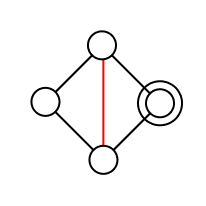
\includegraphics[width=0.4\linewidth]{images/lift-proof1.png}
            \vspace{-1cm}
        \end{minipage}
        \caption{Example of vector diagram $\al$ with extra open cactus in red}
    \end{subfigure}
    \begin{subfigure}[t]{0.5\linewidth}
        \centering
        \begin{minipage}[c][3.8cm][c]{\linewidth}
            \centering
            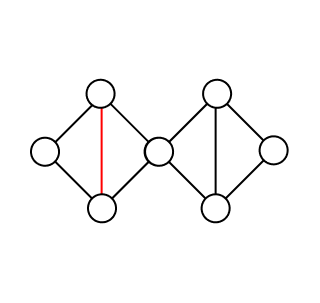
\includegraphics[width=0.5\linewidth]{images/lift-proof2.png}
            \vspace{-1cm}
        \end{minipage}
        \caption{Lift of $\alpha$ at the root (\cref{eq:lift-proof1})}
    \end{subfigure}

    \vspace{-0.5cm}
    \begin{subfigure}[t]{0.45\linewidth}
    \centering
    \begin{minipage}[c][4.2cm][c]{\linewidth}
        \centering
        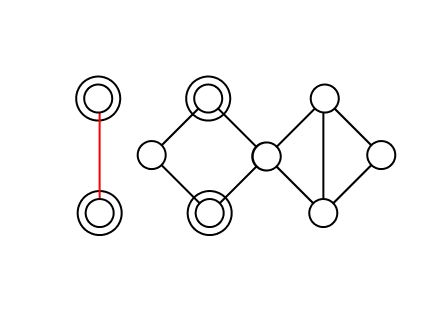
\includegraphics[width=0.6\linewidth]{images/lift-proof3.png}
    \end{minipage}
    \vspace{-1cm}
    \caption{Separate out open cactus (\cref{eq:lift-proof2})}
    \end{subfigure}
    \begin{subfigure}[t]{0.5\linewidth}
    \centering
    \begin{minipage}[c][4.2cm][c]{\linewidth}
        \centering
        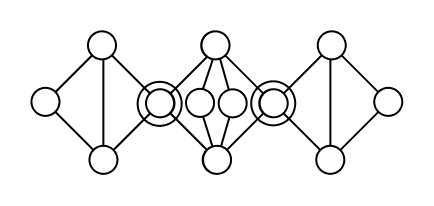
\includegraphics[width=0.6\linewidth]{images/lift-proof4.png}
    \end{minipage}
    \vspace{-1cm}
    \caption{Lift again. The left and right sides are copies of $\al$ while the inner part is 2-edge-connected (\cref{eq:lift-proof3}).}
    \end{subfigure}
    \vspace{1em}
    \caption{Illustration of the main diagrammatic manipulations in the proof of~\cref{prop:Z-support-vector}.}
    \label{fig:lift-proof}
\end{figure}

\subsection{Support of the \texorpdfstring{$w$}{w}-basis}

In this subsection we prove the second part
of~\Cref{thm:universality-new}:

\begin{proposition}
    \label{prop:W-support}
    Suppose that $\bH$ satisfies~\cref{eq:assNorm,eq:assOpen,eq:assOne}. Then for any $\alpha\in \calA\setminus \calE$,
    \[
        \frac 1n |w_\alpha(\bA)|\le \frac 1 {\sqrt n} \cdot (1 + \eps \sqrt n)^{O(1)}\,.
    \]
\end{proposition}

These calculations are simpler than the previous ones, but this is also the point in the proof of~\Cref{thm:universality-new} where puncturing is essential (note that it was not used at all in the previous section, and indeed those results apply equally well to the original $\bH$ or the puncturing $\bA$).

But, without puncturing, the values of graph polynomials that contain bridges can fail to be universal.
For instance, when $\alpha$ is the degree-$d$ star,
Walsh--Hadamard matrices $\bH = \bH^{(n)}$ satisfy
$w_\alpha(\bH) = \Theta(n^{d/2})$, so the limiting traffic distribution does not even exist when $d\ge 3$.
As~\Cref{prop:W-support} shows, puncturing effectively forces all such diagrams to vanish in the traffic distribution.

To prove~\Cref{prop:W-support}, we will isolate a
bridge edge in the graph, and show by induction over the tree of 2-edge-connected components that:

\begin{lemma}
    \label{lem:AW-all}
    For all $\alpha\in \calA_1$,
    \[
       \|\bA \bw_\alpha(\bA)\|_2 \le (1 + \eps \sqrt n)^{O(1)}\,.
    \]
\end{lemma}

\begin{proof}[Proof of~\Cref{prop:W-support} from~\Cref{lem:AW-all}]
    Decompose $\alpha=\alpha_1 \sqcup \alpha_2 \sqcup \{u,v\}$, where $\{u,v\}\in E(\alpha)$ is a bridge edge,
    $\alpha_1\in\calE_1$ is
    rooted at $u$, and
    $\alpha_2\in\calA_1$ is rooted at $v$. Then,
    \[
        |w_\alpha(\bA)| = |\langle \bw_{\alpha_1}(\bA), \bA \bw_{\alpha_2}(\bA)\rangle|\le \|\bw_{\alpha_1}(\bA)\|_2 \|\bA \bw_{\alpha_2}(\bA)\|_2 \le \sqrt n \cdot (1 + \eps \sqrt n)^{O(1)}\,,
    \]
    using~\Cref{thm:fundamental-theorem} on
    the first term
    and~\Cref{lem:AW-all} on the second.
\end{proof}

We prove~\Cref{lem:AW-all} by first treating 
the cactus special case
(\Cref{lem:AW-cactus}), then the 
2-edge-connected special case
(\Cref{lem:AW-2ec}), and then finally the general case by the induction mentioned above.

\begin{lemma}
    \label{lem:AW-cactus}
    For any $\alpha\in\calC_1$,
    \[
        \left\|\bA \bw_\alpha(\bA)\right\|_2\le O(1 + \eps \sqrt n)\,.
    \]
\end{lemma}

\begin{proof}
    We first decompose $\bw_\alpha(\bmA)$ as:
    \[
        \bw_\alpha(\bmA) =  (\bw_\alpha(\bmA) - \bw_\alpha(\bmH)) + \bm \Pi \bw_\alpha(\bmH) + \frac 1n \langle \bm 1, \bw_\alpha(\bmH)\rangle \bm 1\,.
    \]
    Since $\bmA \bm 1 = 0$ and $\|\bmA \|\le 1$
    by assumption, by the triangle inequality we have
    \[
        \|\bmA \bw_\alpha(\bmA)\|_2 \le \|\bw_\alpha(\bmA) - \bw_\alpha(\bmH)\|_2 + \|\bm \Pi \bw_\alpha(\bmH)\|_2\,.
    \]
    By~\Cref{cor:cactus-puncturing-same}, the first
    term is $O(1)$, and by our assumption in~\cref{eq:assOne}, the second term is at most $\eps \sqrt n$.
\end{proof}

\begin{lemma}
    \label{lem:AW-2ec}
    For all $\alpha\in\calE_1$,
    \[
        \|\bA \bw_\alpha(\bA)\|_2\le O(1 + \eps \sqrt n)\,.
    \]
\end{lemma}

\begin{proof}
    We proceed by induction on $|V(\alpha)|$.
    For $\alpha\in\calC_1$ (in particular, if $\alpha$ has only one vertex, which is our base case), the claim
    follows from~\Cref{lem:AW-cactus}.
    For $\alpha\in \calE_1\setminus \calC_1$, 
    we apply~\Cref{prop:open-cactus-decomposition}: there is an open cactus $\sigma$
    induced in $\alpha$ such that removing the
    internal vertices and edges from $\sigma$
    leaves $\alpha$ rooted and 2-edge-connected.
    Let $\{s,t\}$ be the endpoints of $\sigma$,
    and $\beta$ be the graph obtained from $\alpha$ by merging $s$ and $t$. Then, we
    can decompose:
    \[
        \bw_\alpha(\bA) = \bw_\alpha^{s\neq t}(\bA) + \bw_\beta(\bA)\,.
    \]
    On the one hand, $\beta\in\calE_1$ by~\Cref{lem:contract-2ec} 
    and has strictly less vertices than $\alpha$,
    so by induction
    \[
        \|\bA \bw_\beta(\bA)\|_2\le O(1 + \eps \sqrt n)\,.
    \]
    On the other hand, by~\Cref{prop:Z-support-vector},
    \[
        \|\bw_\alpha^{s\neq t}(\bmA)\|_2\le O(1 + \eps \sqrt n)\,.
    \]
    Putting everything together and using $\|\bmA\|\le 1$ and the triangle inequality, we obtain
    \[
        \|\bA \bw_\alpha(\bA)\|_2\le O(1 + \eps \sqrt n)\,,
    \]
    which concludes the induction.
\end{proof}

\begin{lemma}
    \label{lem:new-2ec-construction}
    Let $\al\in\calE$, $v \in V(\al)$, and
    $S$ the set of edges adjacent to $v$ in
    $\alpha$.
    Then there exists $\beta\in\calE$ and $v_1, v_2 \in V(\beta)$ such that
    \begin{align*}
        V(\beta) &= (V(\alpha)\setminus \{v\}) \cup \{v_1, v_2\}\,,\\
        E(\beta) &= (E(\alpha)\setminus S)\cup \phi(S)\cup \{\{v_1, v_2\}\}\,,
    \end{align*}
    where $\phi(e)\in \{\{v_1, u\}, \{v_2, u\}\}$ for all $e=\{v,u\}\in S$.
\end{lemma}

\begin{proof}
    We use the ear decomposition construction
    from the proof of~\Cref{lem:ear-decomposition-lemma}.
    Consider the step of the ear decomposition which adds $v$. During this step, $v$ is a new interior vertex of a path or cycle added to $\al$.
    We define $\beta$ by splitting $v$ into two vertices $v_1, v_2$ with a new edge between them.
    When other ears attach to $v$ in $\al$, we can attach them to either $v_1$ or $v_2$ in $\beta$.
    This process yields an ear decomposition for $\beta$, hence $\beta$ is also 2-edge-connected.
\end{proof}

\begin{proof}[Proof of~\Cref{lem:AW-all}]
    We proceed by induction on the number of
    2-edge-connected components in $\alpha$. If $\alpha$ is
    2-edge-connected, then the result 
    follows by~\Cref{lem:AW-2ec}. We assume
    from now on that $\alpha$ is not 2-edge-connected.

    Let $C$ be the 2-edge-connected component of the root of $\alpha$. Let $\beta_1, \ldots, \beta_k$ 
    ($k\ge 1$) be the 
    connected components disjoint from $\beta$ in 
    the graph obtained
    after removing $E(C)$ and all bridges
    incident to $C$. We root $\beta_i$ at the
    (unique) vertex of $V(\beta_i)$ adjacent to $\beta$. We also consider
    $u_1\in V(\alpha)$, the unique vertex in $V(C)$
    that is adjacent to $V(\beta_1)$.

    Let $\beta\in\calA_2$ be the graph obtained
    from $\alpha$ by adding a second root at $u_1$, and deleting $V(\beta_1)$, $E(\beta_1)$, and the bridge between $u_1$ and $\beta_1$.
    Then, for $i = 2, \ldots, k$, we
    iteratively apply the graph transformation from~\Cref{lem:new-2ec-construction},
    label the new edge $e=\{v_1,v_2\}$ by $\bm A_e = \text{diag}(\bm A \bm w_{\beta_i}(\bmA))$, and transfer the old labels for all
    other edges. In this way, we obtain
    a 2-edge-connected graph $\beta'\in\calE_2$ and a family of matrices $\bm \calA = (\bm A_{e})_{e\in E(\beta')}$ such that \[\bW_{\beta'}(\bm \calA) = \bW_{\beta}(\bA)\,.\] All involved matrices $\bA_e\in\bm \calA$ are either $\bm A$ or of the form 
    $\text{diag}(\bm A \bm w_{\beta_i}(\bmA))$ for some $i\in \{2, \ldots, k\}$, so they
    satisfy
    $\|\bA_e\|\le (1 + \eps \sqrt n)^{O(1)}$ by induction.
    Next, applying~\Cref{thm:fundamental-theorem}, we get
    \[
        \|\bW_\beta(\bA)\| = \|\bW_{\beta'}(\bm \calA)\|\le (1 + \eps \sqrt n)^{O(1)}\,.
    \]
    As a result,
    \[
        \|\bA \bw_\alpha(\bA)\|_2 = \|\bA \bW_\beta(\bA) \bA \bw_{\beta_1}(\bA)\|_2\le \|\bA\| \cdot \|\bW_\beta(\bA)\| \cdot \|\bA \bw_{\beta_1}(\bA)\|_2 \le (1 + \eps \sqrt n)^{O(1)}\,,
    \]
    using again induction on $\|\bA \bw_{\beta_1}(\bA)\|_2$. This concludes the induction.
\end{proof}

\subsection{Putting everything together\texorpdfstring{: Proof of~\Cref{thm:universality-new}}{}}

\begin{proof}[Proof of~\Cref{thm:universality-new}]
    The first part
    follows from~\Cref{prop:Z-support}, and  the second part
    follows from~\Cref{prop:W-support}.
    For the third part, suppose that $\bH$ satisfies~\cref{eq:assNorm,eq:assOpen,eq:assOne} with $\eps^{(n)} = n^{-\frac 12 + o(1)}$. Summarizing, we know that:
    \begin{enumerate}
        \item For all $\sigma\in\calC$, $\frac 1n w_\sigma(\bA)\underset{n\to\infty}{\longrightarrow} m_\sigma\in \R$ by
        assumption.
        \item For all $\alpha\in\calE\setminus \calC$, $\frac 1n z_\alpha(\bA)\underset{n\to\infty}{\longrightarrow} 0$ by the first part.
        \item For all $\alpha\in\calA\setminus \calE$, $\frac 1n w_\alpha(\bA)\underset{n\to\infty}{\longrightarrow} 0$ by the second part.
    \end{enumerate}
    By~\Cref{lem:eqDiffMobius}, the traffic distribution
    of $\bA$ then exists and is uniquely determined
    by $\{m_\sigma : \sigma\in \calC\}$, completing the proof.
\end{proof}
